\documentclass[journal,12pt,twocolumn]{IEEEtran}
\usepackage{setspace}
\usepackage{gensymb}
\singlespacing
\usepackage[cmex10]{amsmath}
\usepackage{amsthm}
\usepackage{mathrsfs}
\usepackage{txfonts}
\usepackage{stfloats}
\usepackage{bm}
\usepackage{cite}
\usepackage{cases}
\usepackage{subfig}
\usepackage{longtable}
\usepackage{multirow}
\usepackage{enumitem}
\usepackage{mathtools}
\usepackage{tikz}
\usepackage{circuitikz}
\usepackage{verbatim}
\usepackage[breaklinks=true]{hyperref}
\usepackage{tkz-euclide} % loads  TikZ and tkz-base
\usepackage{listings}
\usepackage{color}    
\usepackage{array}    
\usepackage{longtable}
\usepackage{calc}     
\usepackage{multirow} 
\usepackage{hhline}   
\usepackage{ifthen}   
\usepackage{lscape}     
\usepackage{chngcntr}
\DeclareMathOperator*{\Res}{Res}
\renewcommand\thesection{\arabic{section}}
\renewcommand\thesubsection{\thesection.\arabic{subsection}}
\renewcommand\thesubsubsection{\thesubsection.\arabic{subsubsection}}

\renewcommand\thesectiondis{\arabic{section}}
\renewcommand\thesubsectiondis{\thesectiondis.\arabic{subsection}}
\renewcommand\thesubsubsectiondis{\thesubsectiondis.\arabic{subsubsection}}
\renewcommand\thetable{\arabic{table}}
% correct bad hyphenation here
\hyphenation{op-tical net-works semi-conduc-tor}
\def\inputGnumericTable{}                                 %%

\lstset{
%language=C,
frame=single, 
breaklines=true,
columns=fullflexible
}
%\lstset{
%language=tex,
%frame=single, 
%breaklines=true
%}

\begin{document}
\newtheorem{theorem}{Theorem}[section]
\newtheorem{problem}{Problem}
\newtheorem{proposition}{Proposition}[section]
\newtheorem{lemma}{Lemma}[section]
\newtheorem{corollary}[theorem]{Corollary}
\newtheorem{example}{Example}[section]
\newtheorem{definition}[problem]{Definition}
\newcommand{\BEQA}{\begin{eqnarray}}
\newcommand{\EEQA}{\end{eqnarray}}
\newcommand{\define}{\stackrel{\triangle}{=}}
\bibliographystyle{IEEEtran}
\providecommand{\mbf}{\mathbf}
\providecommand{\pr}[1]{\ensuremath{\Pr\left(#1\right)}}
\providecommand{\qfunc}[1]{\ensuremath{Q\left(#1\right)}}
\providecommand{\sbrak}[1]{\ensuremath{{}\left[#1\right]}}
\providecommand{\lsbrak}[1]{\ensuremath{{}\left[#1\right.}}
\providecommand{\rsbrak}[1]{\ensuremath{{}\left.#1\right]}}
\providecommand{\brak}[1]{\ensuremath{\left(#1\right)}}
\providecommand{\lbrak}[1]{\ensuremath{\left(#1\right.}}
\providecommand{\rbrak}[1]{\ensuremath{\left.#1\right)}}
\providecommand{\cbrak}[1]{\ensuremath{\left\{#1\right\}}}
\providecommand{\lcbrak}[1]{\ensuremath{\left\{#1\right.}}
\providecommand{\rcbrak}[1]{\ensuremath{\left.#1\right\}}}
\theoremstyle{remark}
\newtheorem{rem}{Remark}
\newcommand{\sgn}{\mathop{\mathrm{sgn}}}
\providecommand{\abs}[1]{\left\vert#1\right\vert}
\providecommand{\res}[1]{\Res\displaylimits_{#1}} 
\providecommand{\norm}[1]{\left\lVert#1\right\rVert}
\providecommand{\mtx}[1]{\mathbf{#1}}
\providecommand{\mean}[1]{E\left[ #1 \right]}
\providecommand{\fourier}{\overset{\mathcal{F}}{ \rightleftharpoons}}
\providecommand{\system}[1]{\overset{\mathcal{#1}}{ \longleftrightarrow}}
\newcommand{\solution}{\noindent \textbf{Solution: }}
\newcommand{\cosec}{\,\text{cosec}\,}
\providecommand{\dec}[2]{\ensuremath{\overset{#1}{\underset{#2}{\gtrless}}}}
\newcommand{\myvec}[1]{\ensuremath{\begin{pmatrix}#1\end{pmatrix}}}
\newcommand{\mydet}[1]{\ensuremath{\begin{vmatrix}#1\end{vmatrix}}}
\let\vec\mathbf
\def\putbox#1#2#3{\makebox[0in][l]{\makebox[#1][l]{}\raisebox{\baselineskip}[0in][0in]{\raisebox{#2}[0in][0in]{#3}}}}
     \def\rightbox#1{\makebox[0in][r]{#1}}
     \def\centbox#1{\makebox[0in]{#1}}
     \def\topbox#1{\raisebox{-\baselineskip}[0in][0in]{#1}}
     \def\midbox#1{\raisebox{-0.5\baselineskip}[0in][0in]{#1}}

\vspace{3cm}
\title{Circle Assignment}
\author{Gautam Singh}
\maketitle
\bigskip

\begin{abstract}
    This document contains the solution to Question 13 of 
    Exercise 2 in Chapter 10 of the class 10 NCERT textbook.
\end{abstract}

\begin{enumerate}
    \item Prove that opposite sides of a quadrilateral circumscribing a circle 
    subtend supplementary angles at the centre of the circle.

    \solution We begin by proving a useful lemma.
    \begin{lemma}
        The line joining the centre of the circle to an external point bisects
        the angle subtended by the tangent chord at the centre.
    \end{lemma}
    \begin{proof}
        Refer to Fig. \ref{fig:tangent}, generated using the Python code 
        \texttt{codes/tangent.py}. Set $\vec{O}$ to be the origin. Since 
        $OA \perp AP$,
        \begin{align}
            \vec{A}^\top\brak{\vec{A}-\vec{P}} &= 0 \\
            \implies \vec{A}^\top\vec{P} &= \norm{\vec{A}}^2
            \label{eq:a-p}
        \end{align}
        Similarly,
        \begin{align}
            \vec{B}^\top\vec{P} = \norm{\vec{B}}^2
            \label{eq:b-p}
        \end{align}
        Since $\vec{A}$ and $\vec{B}$ lie on the circle, their norms are equal.
        Thus, from \eqref{eq:a-p} and \eqref{eq:b-p},
        \begin{align}
            \vec{A}^\top\vec{P} = \vec{B}^\top\vec{P}
        \end{align}
        and the lemma follows.
        \begin{figure}[!ht]
            \centering
            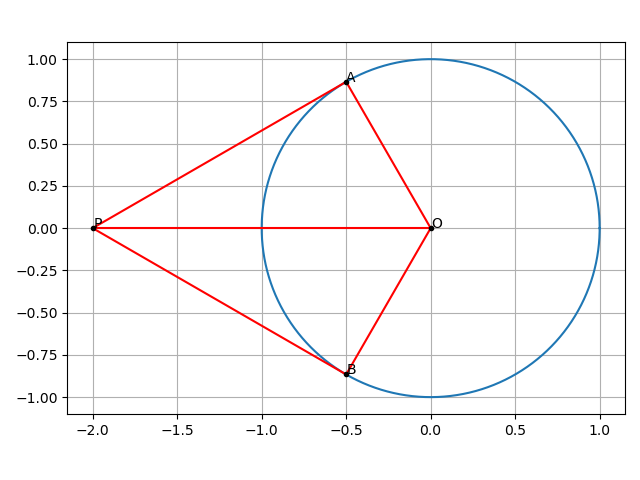
\includegraphics[width=\columnwidth]{figs/tangent.png}
            \caption{$OP$ bisects $\angle AOB$.}
            \label{fig:tangent}
        \end{figure}
    \end{proof}
    Call the quadrilateral $ABCD$, where
    \begin{align}
        \vec{A} = \myvec{-2\\0},\ \vec{C} = \myvec{1\\1}
        \label{eq:a-c-def}
    \end{align}
    Suppose that $ABCD$ circumscribes the unit circle, given by
    \begin{align}
        \vec{x}^\top\vec{x} - 1 = 0
        \label{eq:unit-circ}
    \end{align}
    Comparing \eqref{eq:unit-circ} with the general equation of the circle,
    \begin{align}
        \vec{u} = \vec{0},\ f = -1
        \label{eq:u-f-val}
    \end{align}
    To find the points of contact from $\vec{A}$, we have
    \begin{align}
        \vec{\Sigma_A} &= \brak{\vec{A}+\vec{u}}\brak{\vec{A}+\vec{u}}^\top - \brak{\vec{A}^\top\vec{A}+2\vec{u}^\top\vec{A} + f}\vec{I} \\
                     &= \myvec{1&0\\0&-3}
                     \label{eq:sigma}
    \end{align}
    The eigenparameters of $\vec{\Sigma_A}$ are
    \begin{align}
        \lambda_1 = 1,\ \lambda_2 = -3,\ \vec{P_A} = \vec{I}
        \label{eq:lambda}
    \end{align}
    Thus, the normals to the tangents are
    \begin{align}
        \vec{n_1} = \myvec{1\\\sqrt{3}},\ \vec{n_2} = \myvec{1\\-\sqrt{3}}
        \label{eq:n-sigma}
    \end{align}
    The points of contact are given by
    \begin{align}
        \vec{E} &= -\frac{r\vec{n_2}}{\norm{\vec{n_2}}} - \vec{u} \\
                &= \frac{1}{2}\myvec{-1\\\sqrt{3}} \label{eq:poc-e} \\
        \vec{H} &= -\frac{r\vec{n_1}}{\norm{\vec{n_1}}} - \vec{u} \\
                &= \frac{1}{2}\myvec{-1\\-\sqrt{3}} \label{eq:poc-h}
    \end{align}
    Similarly for $\vec{C}$,
    \begin{align}
        \vec{\Sigma_C} = \myvec{1&1\\1&1} - \vec{I} = \myvec{0&1\\1&0}
    \end{align}
    Notice that
    \begin{align}
        \vec{\Sigma_C}\myvec{1\\1} &= \myvec{1\\1} \\
        \vec{\Sigma_C}\myvec{1\\-1} &= -\myvec{1\\-1} \\
    \end{align}
    Thus, the eigenparameters of $\vec{C}$ are
    \begin{align}
        \mu_1 = 1,\ \mu_2 = -1,\ \vec{P_C} = \myvec{1&1\\1&-1}
    \end{align}
    The normals to the tangents are given by
    \begin{align}
        \vec{m_1} &= \vec{P_C}\myvec{1\\1} = \myvec{2\\0} \\ 
        \vec{m_2} &= \vec{P_C}\myvec{1\\-1} = \myvec{0\\2}
    \end{align}
    Therefore, the points of contact of $\vec{C}$ are
    \begin{align}
        \vec{F} &= \frac{r\vec{m_1}}{\norm{\vec{m_1}}} - \vec{u} \\
                &= \myvec{1\\0} \label{eq:poc-f} \\
        \vec{G} &= \frac{r\vec{m_2}}{\norm{\vec{m_2}}} - \vec{u} \\
                &= \myvec{0\\1} \label{eq:poc-g}
    \end{align}
    Using the lemma we proved above, the direction vectors of $\vec{B}$ and 
    $\vec{D}$ are
    \begin{align}
        \vec{d_B} &= \vec{E} + \vec{F} = \frac{\sqrt{3}}{2}\myvec{\sqrt{3}\\1} \label{eq:d-B} \\
        \vec{d_D} &= \vec{G} + \vec{H} = \frac{1}{2}\myvec{-1\\2-\sqrt{3}} \label{eq:d-D}
    \end{align}
    Clearly,
    \begin{align}
        \norm{\vec{d_B}} &= \sqrt{3} \\
        \norm{\vec{d_D}} &= \sqrt{2-\sqrt{3}}
        \label{eq:norm-d}
    \end{align}
    and from \eqref{eq:a-c-def}, \eqref{eq:d-B} and \eqref{eq:d-D},
    \begin{align}
        \cos\angle AOD &= \frac{\vec{A}^\top\vec{d_D}}{\norm{A}\norm{\vec{d_D}}} \\
                       &= \frac{-1}{2\sqrt{2\sqrt{3}}} \\
                       &= -\frac{\sqrt{2+\sqrt{3}}}{2} \\
                       &= -\frac{\sqrt{3}+1}{2\sqrt{2}} \label{eq:cos-aod} \\
        \cos\angle BOC &= \frac{\vec{C}^\top\vec{d_B}}{\norm{C}\norm{\vec{d_B}}} \\
                       &= \frac{\sqrt{3}+1}{2\sqrt{2}} \label{eq:cos-boc}
    \end{align}
    Hence,
    \begin{align}
        \cos\angle AOD + \cos\angle BOC = 0
    \end{align}
    which implies $\angle AOD + \angle BOC = \pi$, as required.

    The situation is illustrated in Fig. \ref{fig:quad-circ} plotted by the 
    Python code \texttt{codes/quad\_circ.py}. The numerical parameters used 
    in the construction are shown in Table \ref{tab:param}.
    \begin{table}[!ht]
        \centering
        %%%%%%%%%%%%%%%%%%%%%%%%%%%%%%%%%%%%%%%%%%%%%%%%%%%%%%%%%%%%%%%%%%%%%%
%%                                                                  %%
%%  This is the header of a LaTeX2e file exported from Gnumeric.    %%
%%                                                                  %%
%%  This file can be compiled as it stands or included in another   %%
%%  LaTeX document. The table is based on the longtable package so  %%
%%  the longtable options (headers, footers...) can be set in the   %%
%%  preamble section below (see PRAMBLE).                           %%
%%                                                                  %%
%%  To include the file in another, the following two lines must be %%
%%  in the including file:                                          %%
%%        \def\inputGnumericTable{}                                 %%
%%  at the beginning of the file and:                               %%
%%        \input{name-of-this-file.tex}                             %%
%%  where the table is to be placed. Note also that the including   %%
%%  file must use the following packages for the table to be        %%
%%  rendered correctly:                                             %%
%%    \usepackage[latin1]{inputenc}                                 %%
%%    \usepackage{color}                                            %%
%%    \usepackage{array}                                            %%
%%    \usepackage{longtable}                                        %%
%%    \usepackage{calc}                                             %%
%%    \usepackage{multirow}                                         %%
%%    \usepackage{hhline}                                           %%
%%    \usepackage{ifthen}                                           %%
%%  optionally (for landscape tables embedded in another document): %%
%%    \usepackage{lscape}                                           %%
%%                                                                  %%
%%%%%%%%%%%%%%%%%%%%%%%%%%%%%%%%%%%%%%%%%%%%%%%%%%%%%%%%%%%%%%%%%%%%%%



%%  This section checks if we are begin input into another file or  %%
%%  the file will be compiled alone. First use a macro taken from   %%
%%  the TeXbook ex 7.7 (suggestion of Han-Wen Nienhuys).            %%
\def\ifundefined#1{\expandafter\ifx\csname#1\endcsname\relax}


%%  Check for the \def token for inputed files. If it is not        %%
%%  defined, the file will be processed as a standalone and the     %%
%%  preamble will be used.                                          %%
\ifundefined{inputGnumericTable}

%%  We must be able to close or not the document at the end.        %%
	\def\gnumericTableEnd{\end{document}}


%%%%%%%%%%%%%%%%%%%%%%%%%%%%%%%%%%%%%%%%%%%%%%%%%%%%%%%%%%%%%%%%%%%%%%
%%                                                                  %%
%%  This is the PREAMBLE. Change these values to get the right      %%
%%  paper size and other niceties.                                  %%
%%                                                                  %%
%%%%%%%%%%%%%%%%%%%%%%%%%%%%%%%%%%%%%%%%%%%%%%%%%%%%%%%%%%%%%%%%%%%%%%

	\documentclass[12pt%
			  %,landscape%
                    ]{report}
       \usepackage[latin1]{inputenc}
       \usepackage{fullpage}
       \usepackage{color}
       \usepackage{array}
       \usepackage{longtable}
       \usepackage{calc}
       \usepackage{multirow}
       \usepackage{hhline}
       \usepackage{ifthen}

	\begin{document}


%%  End of the preamble for the standalone. The next section is for %%
%%  documents which are included into other LaTeX2e files.          %%
\else

%%  We are not a stand alone document. For a regular table, we will %%
%%  have no preamble and only define the closing to mean nothing.   %%
    \def\gnumericTableEnd{}

%%  If we want landscape mode in an embedded document, comment out  %%
%%  the line above and uncomment the two below. The table will      %%
%%  begin on a new page and run in landscape mode.                  %%
%       \def\gnumericTableEnd{\end{landscape}}
%       \begin{landscape}


%%  End of the else clause for this file being \input.              %%
\fi

%%%%%%%%%%%%%%%%%%%%%%%%%%%%%%%%%%%%%%%%%%%%%%%%%%%%%%%%%%%%%%%%%%%%%%
%%                                                                  %%
%%  The rest is the gnumeric table, except for the closing          %%
%%  statement. Changes below will alter the table's appearance.     %%
%%                                                                  %%
%%%%%%%%%%%%%%%%%%%%%%%%%%%%%%%%%%%%%%%%%%%%%%%%%%%%%%%%%%%%%%%%%%%%%%

\providecommand{\gnumericmathit}[1]{#1} 
%%  Uncomment the next line if you would like your numbers to be in %%
%%  italics if they are italizised in the gnumeric table.           %%
%\renewcommand{\gnumericmathit}[1]{\mathit{#1}}
\providecommand{\gnumericPB}[1]%
{\let\gnumericTemp=\\#1\let\\=\gnumericTemp\hspace{0pt}}
 \ifundefined{gnumericTableWidthDefined}
        \newlength{\gnumericTableWidth}
        \newlength{\gnumericTableWidthComplete}
        \newlength{\gnumericMultiRowLength}
        \global\def\gnumericTableWidthDefined{}
 \fi
%% The following setting protects this code from babel shorthands.  %%
 \ifthenelse{\isundefined{\languageshorthands}}{}{\languageshorthands{english}}
%%  The default table format retains the relative column widths of  %%
%%  gnumeric. They can easily be changed to c, r or l. In that case %%
%%  you may want to comment out the next line and uncomment the one %%
%%  thereafter                                                      %%
\providecommand\gnumbox{\makebox[0pt]}
%%\providecommand\gnumbox[1][]{\makebox}

%% to adjust positions in multirow situations                       %%
\setlength{\bigstrutjot}{\jot}
\setlength{\extrarowheight}{\doublerulesep}

%%  The \setlongtables command keeps column widths the same across  %%
%%  pages. Simply comment out next line for varying column widths.  %%
\setlongtables

\setlength\gnumericTableWidth{%
	63pt+%
	67pt+%
0pt}
\def\gumericNumCols{2}
\setlength\gnumericTableWidthComplete{\gnumericTableWidth+%
         \tabcolsep*\gumericNumCols*2+\arrayrulewidth*\gumericNumCols}
\ifthenelse{\lengthtest{\gnumericTableWidthComplete > \linewidth}}%
         {\def\gnumericScale{1*\ratio{\linewidth-%
                        \tabcolsep*\gumericNumCols*2-%
                        \arrayrulewidth*\gumericNumCols}%
{\gnumericTableWidth}}}%
{\def\gnumericScale{1}}

%%%%%%%%%%%%%%%%%%%%%%%%%%%%%%%%%%%%%%%%%%%%%%%%%%%%%%%%%%%%%%%%%%%%%%
%%                                                                  %%
%% The following are the widths of the various columns. We are      %%
%% defining them here because then they are easier to change.       %%
%% Depending on the cell formats we may use them more than once.    %%
%%                                                                  %%
%%%%%%%%%%%%%%%%%%%%%%%%%%%%%%%%%%%%%%%%%%%%%%%%%%%%%%%%%%%%%%%%%%%%%%

\ifthenelse{\isundefined{\gnumericColA}}{\newlength{\gnumericColA}}{}\settowidth{\gnumericColA}{\begin{tabular}{@{}p{63pt*\gnumericScale}@{}}x\end{tabular}}
\ifthenelse{\isundefined{\gnumericColB}}{\newlength{\gnumericColB}}{}\settowidth{\gnumericColB}{\begin{tabular}{@{}p{67pt*\gnumericScale}@{}}x\end{tabular}}

\begin{tabular}[c]{%
	b{\gnumericColA}%
	b{\gnumericColB}%
	}

%%%%%%%%%%%%%%%%%%%%%%%%%%%%%%%%%%%%%%%%%%%%%%%%%%%%%%%%%%%%%%%%%%%%%%
%%  The longtable options. (Caption, headers... see Goosens, p.124) %%
%	\caption{The Table Caption.}             \\	%
% \hline	% Across the top of the table.
%%  The rest of these options are table rows which are placed on    %%
%%  the first, last or every page. Use \multicolumn if you want.    %%

%%  Header for the first page.                                      %%
%	\multicolumn{2}{c}{The First Header} \\ \hline 
%	\multicolumn{1}{c}{colTag}	%Column 1
%	&\multicolumn{1}{c}{colTag}	\\ \hline %Last column
%	\endfirsthead

%%  The running header definition.                                  %%
%	\hline
%	\multicolumn{2}{l}{\ldots\small\slshape continued} \\ \hline
%	\multicolumn{1}{c}{colTag}	%Column 1
%	&\multicolumn{1}{c}{colTag}	\\ \hline %Last column
%	\endhead

%%  The running footer definition.                                  %%
%	\hline
%	\multicolumn{2}{r}{\small\slshape continued\ldots} \\
%	\endfoot

%%  The ending footer definition.                                   %%
%	\multicolumn{2}{c}{That's all folks} \\ \hline 
%	\endlastfoot
%%%%%%%%%%%%%%%%%%%%%%%%%%%%%%%%%%%%%%%%%%%%%%%%%%%%%%%%%%%%%%%%%%%%%%

\hhline{|-|-}
	 \multicolumn{1}{|p{\gnumericColA}|}%
	{\gnumericPB{\centering}\gnumbox{\textbf{Parameter}}}
	&\multicolumn{1}{p{\gnumericColB}|}%
	{\gnumericPB{\centering}\gnumbox{\textbf{Value}}}
\\
\hhline{|--|}
	 \multicolumn{1}{|p{\gnumericColA}|}%
	{\gnumericPB{\centering}\gnumbox{$r$}}
	&\multicolumn{1}{p{\gnumericColB}|}%
	{\gnumericPB{\centering}\gnumbox{1}}
\\
\hhline{|--|}
	 \multicolumn{1}{|p{\gnumericColA}|}%
     {\gnumericPB{\centering}\gnumbox{$\vec{A}$}}
	&\multicolumn{1}{p{\gnumericColB}|}%
    {\gnumericPB{\centering}\gnumbox{$\myvec{-2\\0}$}}
\\
\hhline{|--|}
	 \multicolumn{1}{|p{\gnumericColA}|}%
     {\gnumericPB{\centering}\gnumbox{$\vec{C}$}}
	&\multicolumn{1}{p{\gnumericColB}|}%
    {\gnumericPB{\centering}\gnumbox{$\myvec{1\\1}$}}
\\
\hhline{|-|-|}
\end{tabular}

\ifthenelse{\isundefined{\languageshorthands}}{}{\languageshorthands{\languagename}}
\gnumericTableEnd

        \caption{Parameters used in the construction of Fig. \ref{fig:quad-circ}.}
        \label{tab:param}
    \end{table}
    \begin{figure}[!ht]
        \centering
        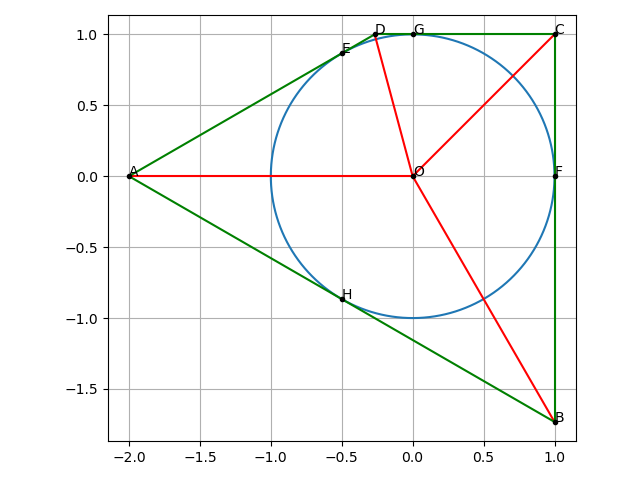
\includegraphics[width=\columnwidth]{figs/quad_circ.png}
        \caption{Angles subtended by the opposite sides of a circumscribing quadrilateral at the center of its incircle are supplementary.}
        \label{fig:quad-circ}
    \end{figure}
\end{enumerate}
\end{document}
